\chapter{GPGPU-Based Implementation of a finite difference algorithm}

\section{Introduction}

Now that we have given an introduction to the theoretical and numerical aspects of the thesis,
the object of this section is to give an overview of the implemenation of an algorithm using finite difference schemes.
The source code used for the computations is based on an existing version from [A.Tilgner].
It was furthermore optimized  and extended by the immersed boundary methods, which will be explained in more detail in chapter (5.).
Especially in this context we will introduce some aspects of GPGPU\footnote{General Purpose Computation on Graphics Processing Unit - Allg.  Bezeichung für Allzweck-Berechnungen auf Grafikprozessoren}-Computing
with the CUDA \footnote{Computing Uniform Device Architecture} architecture.
For the computations the  Tesla C1060 and Tesla K20m GPUs by NVIDIA were used, the complete system configurations can be looked up at (AX.X).

\section{GPGPU-Computing with CUDA}

CUDA is an architecture developed by NVIDIA to enable an easy approach to the Implementation of GPGPU-based algorithms.
The underlying idea is to hide the complexity of the hardware under a more high oriented and generalized software abstraction layer.
This is done by introducing some additional programming language extensions i.e. in c/c++\footnote{WIR BENUTZEN C/C++ /PYTHON ETC},
furthermore it is necessary to use a CUDA suited compiler like NVCC.

\subsection{Hardware and Memory Architecture}

A cuda device contains an array of so called streaming multiprocessors (SM).
Each of these SMs contains a group of small execution units, which are called cuda cores.
For the exchange of data between different SMs, cuda cores and the CPU side of the computer, there exists different
types of memory, as shown  in figure (X).

\begin{figure}[!bp]
  \centering
  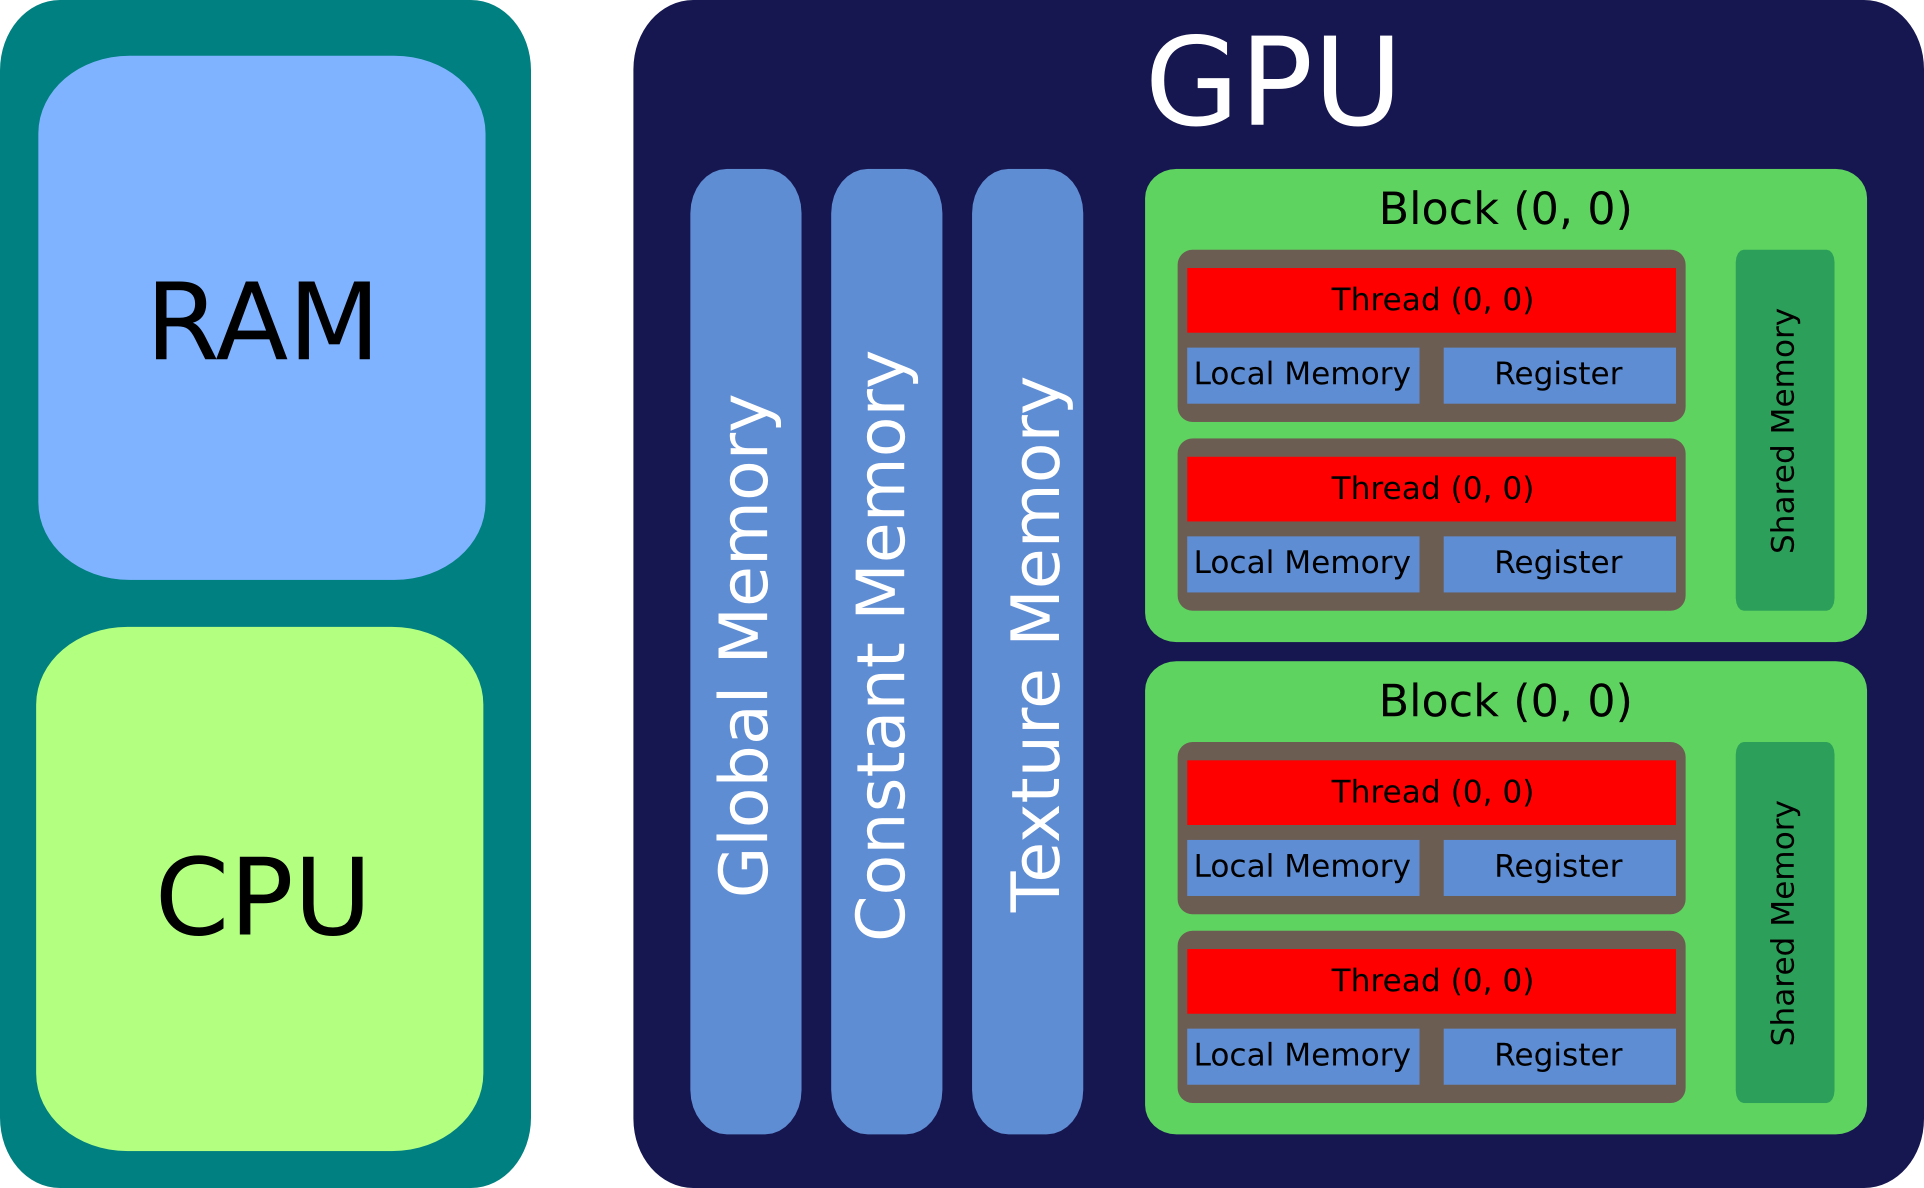
\includegraphics[width=0.8\textwidth]{gfx/cuda/gpu.png}\label{fig:gpu_arch}
  \caption{Memory layout of a Nvidia-GPU}
\end{figure}

\begin{description}
    \item[Global Memory] The global memory is the largest memory on the gpu and can be accessed by all cuda cores.
                         It is  used to exchange data with the RAM and distribute it between different SMs.
                         Reading from the global memory can be quite slow, therefore different optimization approaches exists,
                         for example the creation of a cached texture- or constant-memory.

    \item[Shared Memory] Each SM contains a shared memory, much smaller than the global memory \footnote{Around 16kb on c1060 and 64kb on k20m}. It is accessible
                         by all cuda cores of the SM.
                         This memory type is much faster (x100) than the global memory and is really usefull when multiple operations
                         by different cuda cores are carried out on the same data.
                         \newpage

    \item[Register / Local Memory] Each cuda core posseses an own set of registers and local memory.
                                   The register access is even slightly faster as on the shared memory. The local memory access is very slow since
                                   it is created on the global memory, when the cuda core runs out of resources.
\end{description}

As a conlusion the algorithm should fulfil the following prerequisites.
The global memory should be used for data transfer and distribution, with as little as possible global reads.
Immediatly after the data is transfered to the shared memory there should be as many as possible computations before transfering
it back. Furthermore all memory accesses should be optimized, see chapter (X.X).

\subsection{CUDA C/C++ API}

The CUDA C/C++ API is an extension of the C programming language.
There exists a different number of versions, supporting a different number of hardware architectures, def by C.
The ???BLABLAalgorithm in our cases uses the compute capability X.X.
A majority of the API functions are so called \textbg{host functions}  which are executed by the CPU.
These functions are used i.e. for storage allocation on the gpu, data transfers and error checking.
For example the function call
\begin{verbatim}
    cudaMalloc((void **) &vx_d, A);
\end{verbatim}
allocates memory with size A at the pointer vx\_d on the device (GPU). As we can see here, the syntax for host functions is still in C.
There are two kinds of function types executed on the device.
The most import are \textbg{global functions}, which are called by the host and executed on the device.
Last but not least there are \textbg{device functions} which are called and executed by the device.
An example of the syntax for defining these kind of functions is given in Appendix (X.X).


The execution of a global function has the following syntax

\begin{verbatim}
    time_step<<<dimGrid,dimBlock>>>(x, y, z);
\end{verbatim}






On the host (CPU) side the API offers a nu





-host functions
-memcpy

-kernel
-   call

example 1d array
-grid layout function call
-blocks
-threadidx etc

\section{Algorithm Implementation}
-oder so ?
-erläuterung  implementierung
-speicherverwaltung


\section{Validierung}
- beispiel rayleigh benard system
- masa
- vgl o2 vs o4 masa cube
- bifurcation

\section{Optimization}
- coalesceded
- bank conflicts?
- teilvolumen nicht rechnen

\newpage

